\begin{frame}{Jagt for stående hund}
    
     \begin{columns}[T]
        \begin{column}{0.58\textwidth}
            \begin{itemize}
                \item \textbf{Aktiv} jagtform – hund med stort søg står stand ved typisk hønsefugl
                \item Typisk solo eller få jægere
                \item Jægeren giver signal til hunden om at lette fuglen ved stand
                \item Der anvendes glatløbet haglgevær til jagtformen
                \item Uddøende jagtform i DK pga. den intensive arealudnyttelse
            \end{itemize}
        \end{column}
        
         \begin{column}{0.4\textwidth}
            \centering
            \vspace{0.5em}
            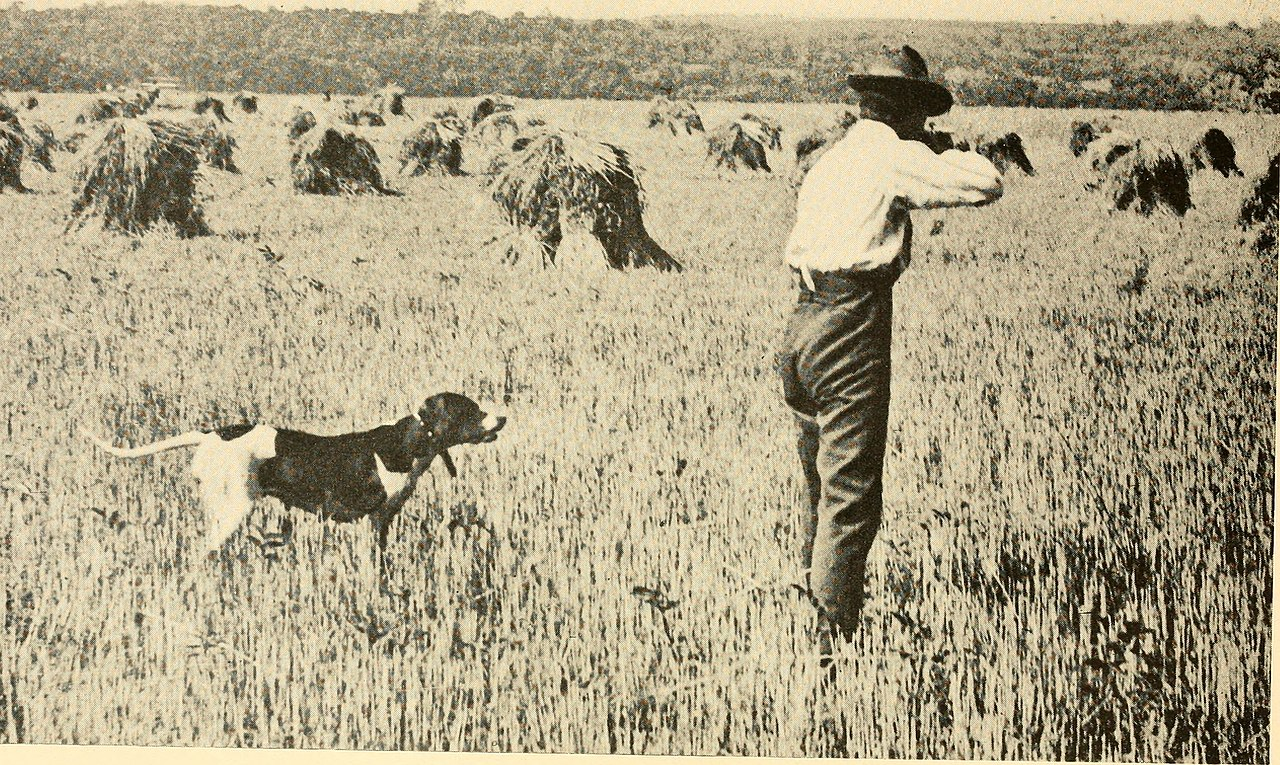
\includegraphics[width=\textwidth,height=0.82\textheight,keepaspectratio]
                {Billeder/Jagtformer/staaende_jagt}
            % Alternativer – fjern kommentartegn hvis du vil skifte:
            % \includegraphics[width=\textwidth]{highseat-snow-forest-hunter.jpg}
            % \includegraphics[width=\textwidth]{hunter-highseat-morning-mist.jpg}
            % \includegraphics[width=\textwidth]{ansitz-jagttarn-skov.jpg}
        \end{column}
    \end{columns}
    
\end{frame}